\documentclass[a4paper]{article}
\usepackage[utf8]{inputenc}
\usepackage[T1]{fontenc}
\usepackage[polish]{babel}
\usepackage{graphicx}
\usepackage{listings}
\usepackage{float}
\usepackage{geometry}
\usepackage{amsmath}


 \geometry{
 a4paper,
 total={160mm,252mm},
 left=25mm,
 top=25mm,
 }


\begin{document}


\begin{titlepage}
    \begin{center}
        \vspace*{1cm}

        \Huge
        \textbf{Modelowanie i symulacje systemów}
        \textbf{HiPUTS - traffic lights}

        \Large
        \vspace{0.5cm}
        Raport 1,2,3

        \vspace{1.5cm}

        \textbf{
        Błażej Nowicki \\
        Przemysław Węglik \\
        }
        

        \vspace{1.8cm}

        \textbf{
        grupa poniedziałek, 13:15 - 14:45
        }

        \vfill
        \vspace{0.8cm}

        
\includegraphics[width=0.4\textwidth]{./imgs/agh_logo.jpg}

        Wydział Informatyki\\
        Akademia Górniczo Hutnicza\\
        Kraków\\
        \today

    \end{center}
\end{titlepage}

\section{Analiza problemu}


\section{Wybór narzędzi}


\section{Pierwsze prace}

\subsection{Bughunt w wizualizacji}

Zaczęliśmy od drobnego uprzątnięcia kodu wizualizacji webowej i naprawy błędu wyświetlania prędkości. Linie oznaczające wektor prędkości auta skalowały się nie odwrotnie proporcjonlanie do kroku czasowego. Po ustawieniu kroku na 0.1 (aby bardziej granularnie móc śledzić ruchy pojazdów) wektory wydłużyły się 10x. Wizualizacja z błędem:

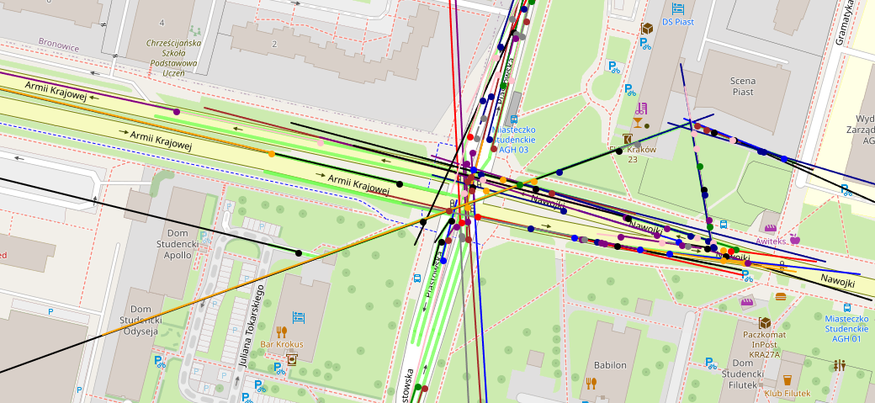
\includegraphics[width=1\textwidth]{./imgs/bug.png}

Błąd rozwiązany:

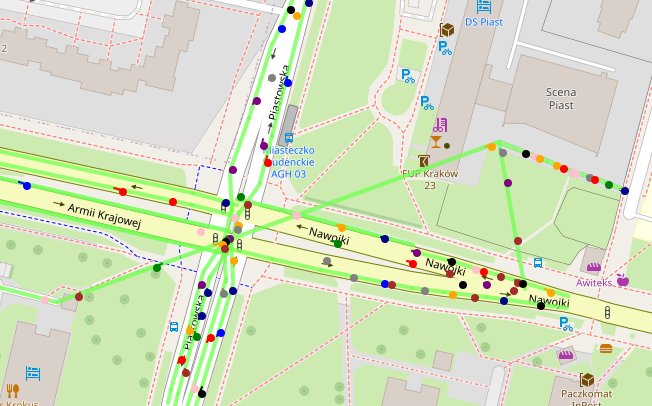
\includegraphics[width=1\textwidth]{./imgs/bug_solved.png}

\subsection{Mapa testowa}

Po rozmowie z poprzednią maintainerką projektu - Natalią ustaliliśmy, że bedziemy potrzebować prostej mapy testowej. Mogą z niej również benefitować inni uczestnicy projektu. Wcześniej (przed dodaniem multilane) działał generator mapy typu grid - torus. Mapa typu grid z połączonymi dołem i górą, oraz prawą i lewą stroną. Niestety modyfikacja kod Javowego na potrzeby multilane okazała się trudna. Zamiast tego stworzyliśmy skrypt pythonowy który generuje mapy osm na podstawie grafów z biblioteki NetworkX. W ten sposób kolejni użytkownicy będą mogli łatwo zedytować skrypt by dodać do mapy testowej przejścia dla pieszych, buspasy itp.

Mapa prezentuje się następująco (wariant grid 3x3, 2 pasy w każdą stronę)


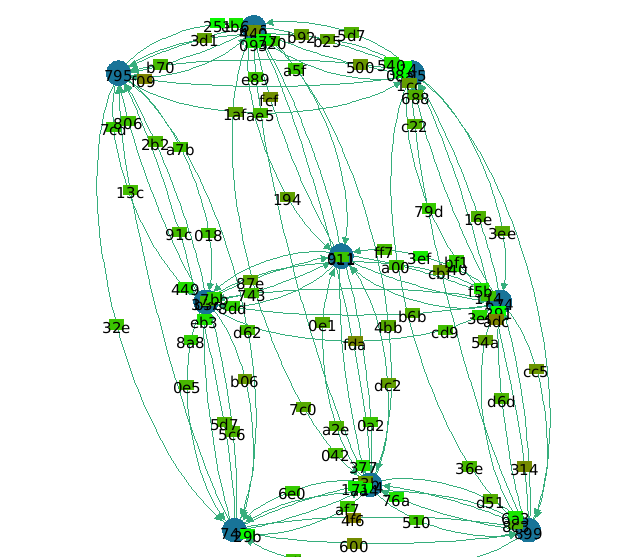
\includegraphics[width=1\textwidth]{./imgs/map1.png}

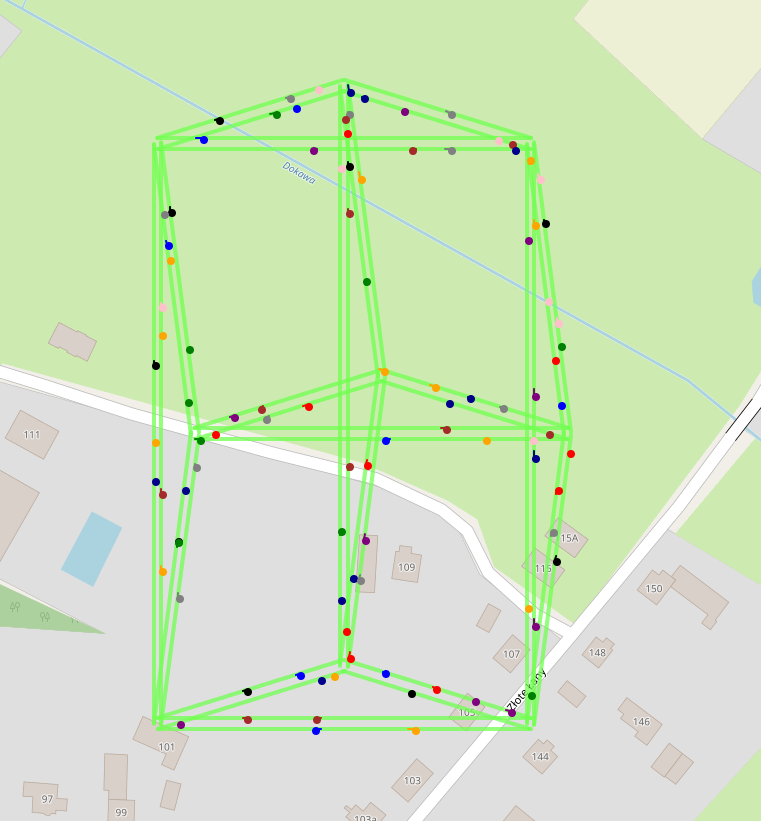
\includegraphics[width=1\textwidth]{./imgs/map2.png}

Część wierzchołków zostałą celowo przesunięta w celu lepszej wizualizacji połączej toroidalnych.

\end{document}